\documentclass{beamer}
\usepackage[utf8]{inputenc}

\usetheme{Madrid}
\usecolortheme{default}
\usepackage{extarrows}
\usepackage{amsmath}
\usepackage{extarrows}
\usepackage{amssymb,amsfonts,amsthm}
\usepackage{txfonts}
\usepackage{tkz-euclide}
\usepackage{listings}
\usepackage{adjustbox}
\usepackage{array}
\usepackage{tabularx}
\usepackage{gvv}
\usepackage{lmodern}
\usepackage{circuitikz}
\usepackage{tikz}
\usepackage{graphicx}
\usepackage{amsmath} 

\setbeamertemplate{page number in head/foot}[totalframenumber]

\usepackage{tcolorbox}
\tcbuselibrary{minted,breakable,xparse,skins}

\definecolor{bg}{gray}{0.95}
\DeclareTCBListing{mintedbox}{O{}m!O{}}{%
  breakable=true,
  listing engine=minted,
  listing only,
  minted language=#2,
  minted style=default,
  minted options={%
    linenos,
    gobble=0,
    breaklines=true,
    breakafter=,,
    fontsize=\small,
    numbersep=8pt,
    #1},
  boxsep=0pt,
  left skip=0pt,
  right skip=0pt,
  left=25pt,
  right=0pt,
  top=3pt,
  bottom=3pt,
  arc=5pt,
  leftrule=0pt,
  rightrule=0pt,
  bottomrule=2pt,
  toprule=2pt,
  colback=bg,
  colframe=orange!70,
  enhanced,
  overlay={%
    \begin{tcbclipinterior}
    \fill[orange!20!white] (frame.south west) rectangle ([xshift=20pt]frame.north west);
    \end{tcbclipinterior}},
  #3,
}
\lstset{
    language=C,
    basicstyle=\ttfamily\small,
    keywordstyle=\color{blue},
    stringstyle=\color{orange},
    commentstyle=\color{green!60!black},
    numbers=left,
    numberstyle=\tiny\color{gray},
    breaklines=true,
    showstringspaces=false,
}
\title %optional
{12.478}
\author 
{EE25BTECH11049-Sai Krishna Bakki}

\begin{document}

\frame{\titlepage}
\begin{frame}{Question}
A force $\vec{P}=\myvec{2\\-5\\6}$ acts on a particle. The particle is moved from point $\vec{A}$ to point $\vec{B}$, where the position vectors of $\vec{A}$ and $\vec{B}$ are $\myvec{6\\1\\-3}$ and $\myvec{4\\-3\\-2}$ respectively. The work done is
\end{frame}
\begin{frame}{Theoretical Solution}
    Given
\begin{align}
    \text{Force } \vec{P}=\myvec{2\\-5\\6},\vec{A}=\myvec{6\\1\\-3},\vec{B}=\myvec{4\\-3\\-2}
\end{align}
Work done is given by
\begin{align}
    \vec{P}^T\brak{\vec{B}-\vec{A}}\\
    \implies \myvec{2&-5&6}\brak{\myvec{4\\-3\\-2}-\myvec{6\\1\\-3}}\\
    \implies \myvec{2&-5&6}\myvec{-2\\-4\\1}\\
    \implies -4+20+6=22
\end{align}
$\therefore$ The work done is 22.
\end{frame}
\begin{frame}[fragile]
\frametitle{C Code}
\begin{lstlisting}
#include <stdio.h>

// Define a structure to hold 3D vector components.
// This structure will be mirrored in the Python script.
typedef struct {
    double x;
    double y;
    double z;
} Vector3D;

double calculate_work_done(const Vector3D* force, const Vector3D* pos_a, const Vector3D* pos_b) {
    // 1. Calculate the displacement vector (d = B - A)
    Vector3D displacement;
    displacement.x = pos_b->x - pos_a->x;
    displacement.y = pos_b->y - pos_a->y;
    displacement.z = pos_b->z - pos_a->z;
\end{lstlisting}
\end{frame}
\begin{frame}[fragile]
\frametitle{C Code}
\begin{lstlisting}
    // 2. Calculate the dot product of Force and Displacement
    double work_done = force->x * displacement.x + 
                       force->y * displacement.y + 
                       force->z * displacement.z;

    return work_done;
}
// This part is not called by Python.
int main() {
    Vector3D force_P    = {2.0, -5.0, 6.0};
    Vector3D position_A = {6.0, 1.0, -3.0};
    Vector3D position_B = {4.0, -3.0, -2.0};
    // Calculate work done by calling the function
    double work = calculate_work_done(&force_P, &position_A, &position_B);
    printf("--- Standalone C Execution ---\n");
    printf("Work Done: %f units\n", work);
   return 0;
}
\end{lstlisting}
\end{frame}
\begin{frame}[fragile]
\frametitle{Python Code Through Shared Output}
\begin{lstlisting}
import ctypes
import os
import platform
import numpy as np
import matplotlib.pyplot as plt
from mpl_toolkits.mplot3d import Axes3D

# --- Step 1: Define a Python class that mirrors the C struct ---
class Vector3D(ctypes.Structure):
    """A ctypes structure to match the Vector3D struct in C."""
    _fields_ = [("x", ctypes.c_double),
                ("y", ctypes.c_double),
                ("z", ctypes.c_double)]

# --- Step 2: Locate and load the compiled C shared library --
# Determine the correct file extension for the shared library based on the OS
system = platform.system()
\end{lstlisting}
\end{frame}
\begin{frame}[fragile]
\frametitle{Python Code Through Shared Output}
\begin{lstlisting}
if system == "Windows":
    lib_extension = ".dll"
elif system == "Darwin": # macOS
    lib_extension = ".dylib"
else: # Linux and other POSIX
    lib_extension = ".so"

lib_name = "force" + lib_extension
lib_path = os.path.join(os.path.dirname(__file__), lib_name)

# Provide instructions and exit if the library is not found
try:
    c_lib = ctypes.CDLL(lib_path)
except OSError:
    print(f"Error: Could not load the shared library '{lib_name}'.")
    print("Please compile the C code into a shared library first.")
    print("\nOn Linux or macOS, use this command in your terminal:")
    \end{lstlisting}
\end{frame}
\begin{frame}[fragile]
\frametitle{Python Code Through Shared Output}
\begin{lstlisting}
    print("gcc -shared -o work_done_calculator.so -fPIC work_done_calculator.c")
    print("\nOn Windows (with MinGW/GCC), use this command:")
    print("gcc -shared -o work_done_calculator.dll work_done_calculator.c")
    exit()

# --- Step 3: Define the C function's signature for ctypes ---

# Get a reference to the function from the loaded library
calculate_work_done_c = c_lib.calculate_work_done

# Specify the argument types (three pointers to Vector3D)
calculate_work_done_c.argtypes = [ctypes.POINTER(Vector3D), 
                                  ctypes.POINTER(Vector3D), 
                                  ctypes.POINTER(Vector3D)]

# Specify the return type (a double)
calculate_work_done_c.restype = ctypes.c_double
\end{lstlisting}
\end{frame}
\begin{frame}[fragile]
\frametitle{Python Code Through Shared Output}
\begin{lstlisting}
# --- Step 4: Prepare data and call the C function ---
# The problem data as tuples
force_P_data    = (2.0, -5.0, 6.0)
position_A_data = (6.0, 1.0, -3.0)
position_B_data = (4.0, -3.0, -2.0)

# Create Python instances of the Vector3D structure
force_P    = Vector3D(*force_P_data)
position_A = Vector3D(*position_A_data)
position_B = Vector3D(*position_B_data)

# Call the C function, passing the structures by reference
work_done = calculate_work_done_c(ctypes.byref(force_P), 
                                  ctypes.byref(position_A), 
                                  ctypes.byref(position_B))
\end{lstlisting}
\end{frame}
\begin{frame}[fragile]
\frametitle{Python Code Through Shared Output}
\begin{lstlisting}
# --- Step 5: Display the result ---

print("--- Calling C function from Python ---")
print(f"Force: {force_P_data}")
print(f"Position A: {position_A_data}")
print(f"Position B: {position_B_data}")
print("-" * 35)
print(f"Work Done (calculated by C library): {work_done} Joules")

# --- Step 6: 3D Visualization using Matplotlib ---
# Convert tuples to NumPy arrays for plotting and vector math
force_np = np.array(force_P_data)
pos_a_np = np.array(position_A_data)
pos_b_np = np.array(position_B_data)
displacement_np = pos_b_np - pos_a_np

# Create the plot
fig = plt.figure(figsize=(10, 8))
ax = fig.add_subplot(111, projection='3d')
\end{lstlisting}
\end{frame}
\begin{frame}[fragile]
\frametitle{Python Code Through Shared Output}
\begin{lstlisting}
# Plotting points A and B
ax.scatter(*pos_a_np, color='blue', s=100, label='Point A')
ax.scatter(*pos_b_np, color='red', s=100, label='Point B')

# Origin for position vectors
origin = [0, 0, 0]

# Position vectors from origin
ax.quiver(*origin, *pos_a_np, color='cyan', arrow_length_ratio=0.1, label='Position Vector A')
ax.quiver(*origin, *pos_b_np, color='magenta', arrow_length_ratio=0.1, label='Position Vector B')

# Displacement vector from A to B
ax.quiver(*pos_a_np, *displacement_np, color='green', arrow_length_ratio=0.1, label='Displacement Vector (d)')
\end{lstlisting}
\end{frame}
\begin{frame}[fragile]
\frametitle{Python Code Through Shared Output}
\begin{lstlisting}
# Force vector acting on the particle (shown at point A for context)
ax.quiver(*pos_a_np, *force_np, color='orange', arrow_length_ratio=0.1, label='Force Vector (P)')
# Setting plot labels and title
ax.set_xlabel('X-axis')
ax.set_ylabel('Y-axis')
ax.set_zlabel('Z-axis')
ax.set_title('3D Visualization of Force and Displacement')

# Setting axis limits
max_val = np.max(np.abs(np.concatenate(([0], pos_a_np, pos_b_np, pos_a_np + displacement_np, pos_a_np + force_np))))
ax.set_xlim([-max_val, max_val])
ax.set_ylim([-max_val, max_val])
ax.set_zlim([-max_val, max_val])
ax.legend()
ax.grid(True)
plt.show()
\end{lstlisting}
\end{frame}
\begin{frame}[fragile]
\frametitle{Python Code}
\begin{lstlisting}
import numpy as np
import matplotlib.pyplot as plt
from mpl_toolkits.mplot3d import Axes3D

# Problem Data based on the image
# Using NumPy arrays for vector operations
force_P = np.array([2, -5, 6])
position_A = np.array([6, 1, -3])
position_B = np.array([4, -3, -2])

# --- Calculation using NumPy ---

# 1. Calculate the displacement vector (d = B - A)
# NumPy allows for direct vector subtraction.
displacement = position_B - position_A

# 2. Calculate the work done (Work = Force · Displacement)
# Using the dot product function from NumPy.
work_done = np.dot(force_P, displacement)
\end{lstlisting}
\end{frame}
\begin{frame}[fragile]
\frametitle{Python Code}
\begin{lstlisting}
# --- Output the result ---
print(f"Force Vector (P): {force_P}")
print(f"Position Vector (A): {position_A}")
print(f"Position Vector (B): {position_B}")
print("-" * 20)
print(f"Calculated Displacement Vector (d): {displacement}")
print(f"Work Done: {work_done} Joules")

# --- 3D Visualization ---
fig = plt.figure(figsize=(10, 8))
ax = fig.add_subplot(111, projection='3d')

# Plotting points A and B
ax.scatter(*position_A, color='blue', s=100, label='Point A')
ax.scatter(*position_B, color='red', s=100, label='Point B')

# Drawing vectors using quiver
# Origin for vectors
origin = [0, 0, 0]
\end{lstlisting}
\end{frame}
\begin{frame}[fragile]
\frametitle{Python Code}
\begin{lstlisting}
# Position vectors from origin
ax.quiver(*origin, *position_A, color='cyan', arrow_length_ratio=0.1, label='Position Vector A')
ax.quiver(*origin, *position_B, color='magenta', arrow_length_ratio=0.1, label='Position Vector B')

# Displacement vector from A to B
ax.quiver(*position_A, *displacement, color='green', arrow_length_ratio=0.1, label='Displacement Vector (d)')

# Force vector acting on the particle (shown at point A for context)
ax.quiver(*position_A, *force_P, color='orange', arrow_length_ratio=0.1, label='Force Vector (P)')
\end{lstlisting}
\end{frame}
\begin{frame}[fragile]
\frametitle{Python Code}
\begin{lstlisting}
# Setting plot labels and title
ax.set_xlabel('X-axis')
ax.set_ylabel('Y-axis')
ax.set_zlabel('Z-axis')
ax.set_title('3D Visualization of Force and Displacement')

# Setting axis limits to be equal for a better aspect ratio
max_val = np.max(np.abs(np.concatenate(([0], position_A, position_B, position_A + force_P))))
ax.set_xlim([-max_val, max_val])
ax.set_ylim([-max_val, max_val])
ax.set_zlim([-max_val, max_val])
ax.legend()
ax.grid(True)

# Show plot
plt.show()
\end{lstlisting}
\end{frame}
\begin{frame}{Plot By C code and Python Code}
    \begin{figure}
    \centering
    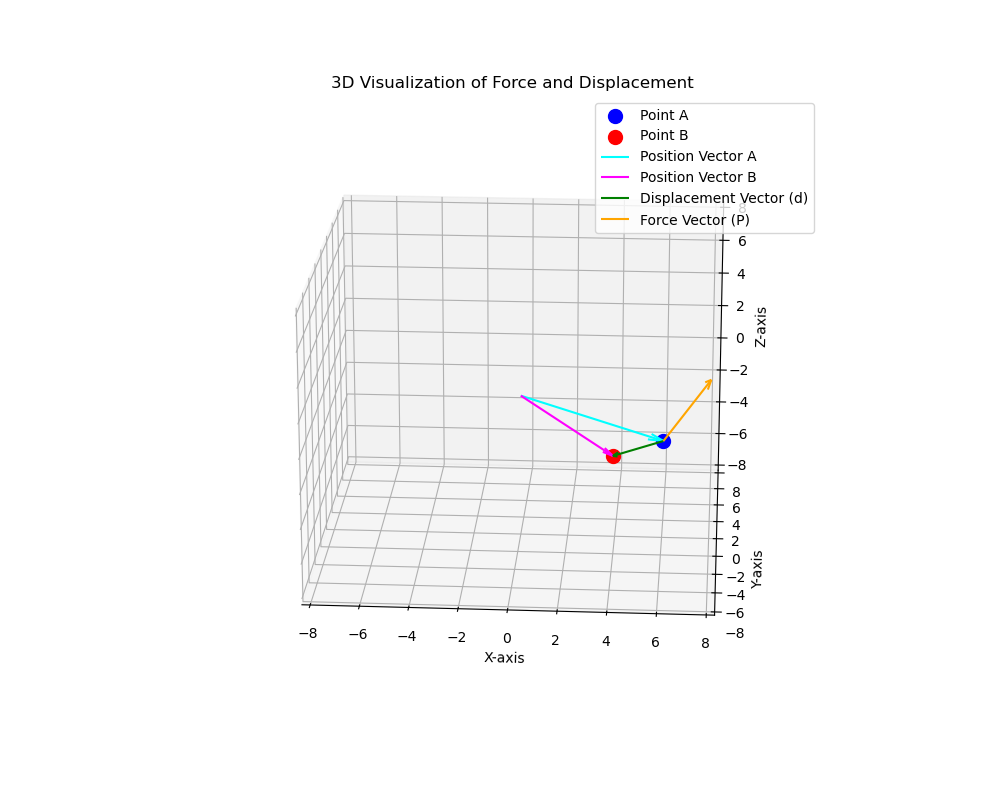
\includegraphics[width=0.7\columnwidth]{figs/Figure_1.png}
    \label{fig:placeholder}
    \caption{1}
\end{figure}
\end{frame}
\end{document}
